\documentclass[xcolor=svgnames]{beamer}
\usepackage[utf8]{inputenc}
\usepackage[english]{babel}
\usepackage{numprint}
\usepackage{booktabs}

\usetheme{Proso}

\newcommand{\head}[1]{\textnormal{\textbf{#1}}}

\title{Systems for Adaptive Practice of Facts}
\author{Jan Papou\v{s}ek}
\institute{Masaryk University Brno}
\date{\today}

\begin{document}
% --------------------------- SLIDE --------------------------------------------
\frame[plain]{\titlepage}
% ------------------------------------------------------------------------------
% --------------------------- SLIDE --------------------------------------------
\begin{frame}
	\frametitle{Systems for Practice}
	\begin{itemize}
		\item learning vs. practice systems
		\item focus on atomic tasks (items)
		\begin{itemize}
			\item \textbf{facts -- vocabulary, location of countries, anatomy}
			\item simple mathematics tasks
			\item estimates -- currency conversion
		\end{itemize}
		\item adaptability in smart question construction
	\end{itemize}
\end{frame}
% ------------------------------------------------------------------------------
% --------------------------- SLIDE --------------------------------------------
\begin{frame}
	\frametitle{slepemapy.cz}
	\begin{center}
		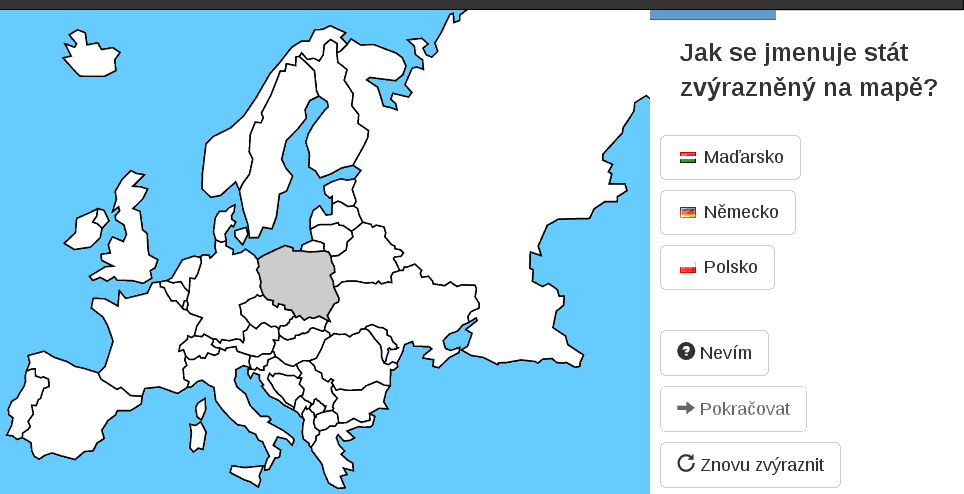
\includegraphics[width=\textwidth]{practice-example-cs.png}
	\end{center}
\end{frame}
% ------------------------------------------------------------------------------
% --------------------------- SLIDE --------------------------------------------
\begin{frame}
	\frametitle{slepemapy.cz}
	\begin{center}
		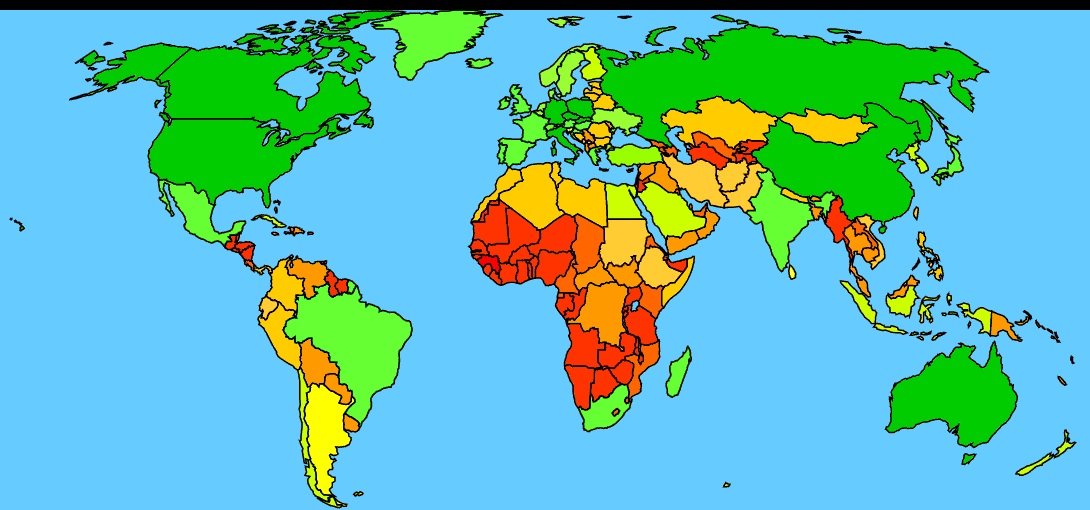
\includegraphics[width=\textwidth]{knowledge-map.png}
	\end{center}
\end{frame}
% ------------------------------------------------------------------------------
% --------------------------- SLIDE --------------------------------------------
\begin{frame}
	\frametitle{slepemapy.cz}
	\begin{itemize}
		\item source of data for research
		\item almost 9 mil. answers
		\item almost \numprint{50000} feedback records
		\item per month:
			\begin{itemize}
				\item 1 mil. answers
				\item \numprint{10000} users
				\item \numprint{10000} feedback records
			\end{itemize}
	\end{itemize}
\end{frame}
% ------------------------------------------------------------------------------
% --------------------------- SLIDE --------------------------------------------
\begin{frame}
	\frametitle{slepemapy.cz -- main parts}
	\begin{enumerate}
		\item predictive model
			\begin{itemize}
				\item estimation of prior knowledge (user) and difficulty (item)
				\item estimation of current knowledge (user, item)
			\end{itemize}
		\item question construction
			\begin{itemize}
				\item item
				\item (question type)
				\item number of options
				\item items in options
			\end{itemize}
	\end{enumerate}
\end{frame}
% ------------------------------------------------------------------------------
% --------------------------- SLIDE --------------------------------------------
\begin{frame}
	\frametitle{Predictive Model: Elo}
	\begin{itemize}
		\item rating of chess players
		\item player 1 vs. player 2\\ $\rightarrow$ student ($\theta$) vs. item ($d$)
		\item update, $R \in \{0, 1\}$, $E(R) \in [0, 1]$
		 \begin{itemize}
			\item $ \theta := \theta + K \cdot (R - E(R))$
			\item $ d := d - K \cdot (R - E(R))$
		 \end{itemize}
	\end{itemize}
\end{frame}
% ------------------------------------------------------------------------------
% --------------------------- SLIDE --------------------------------------------
\begin{frame}
	\frametitle{Question Construction: Item}
	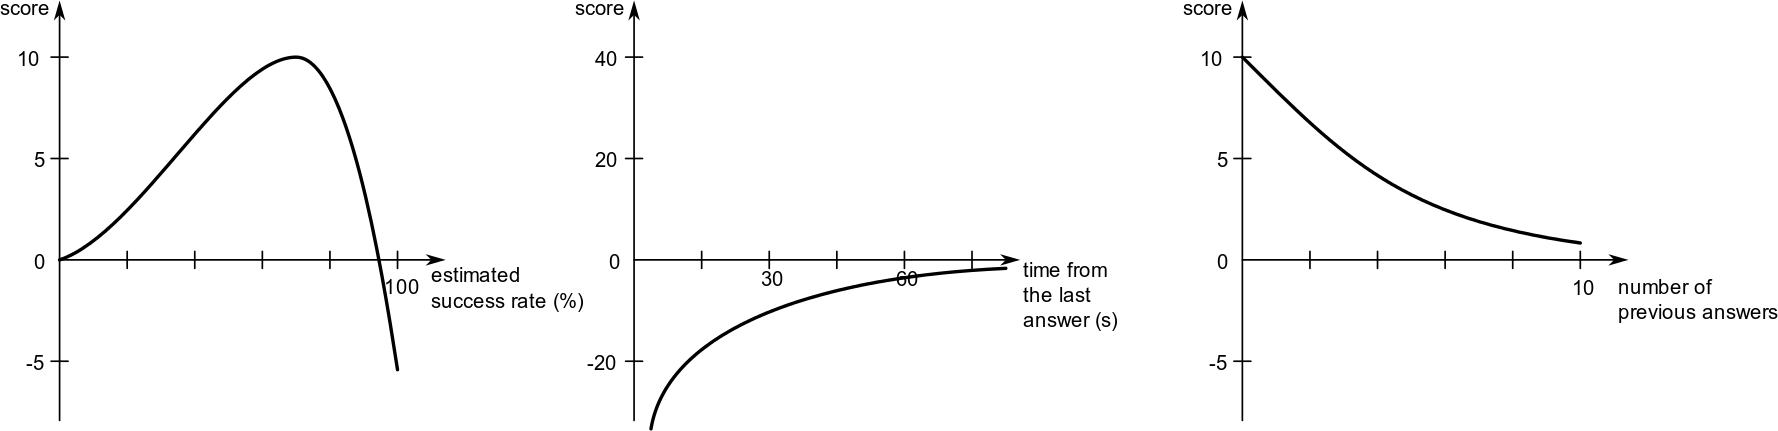
\includegraphics[width=\textwidth]{score-functions}
\end{frame}
% ------------------------------------------------------------------------------
% --------------------------- SLIDE --------------------------------------------
\begin{frame}
	\frametitle{Question Construction: Target Difficulty}
	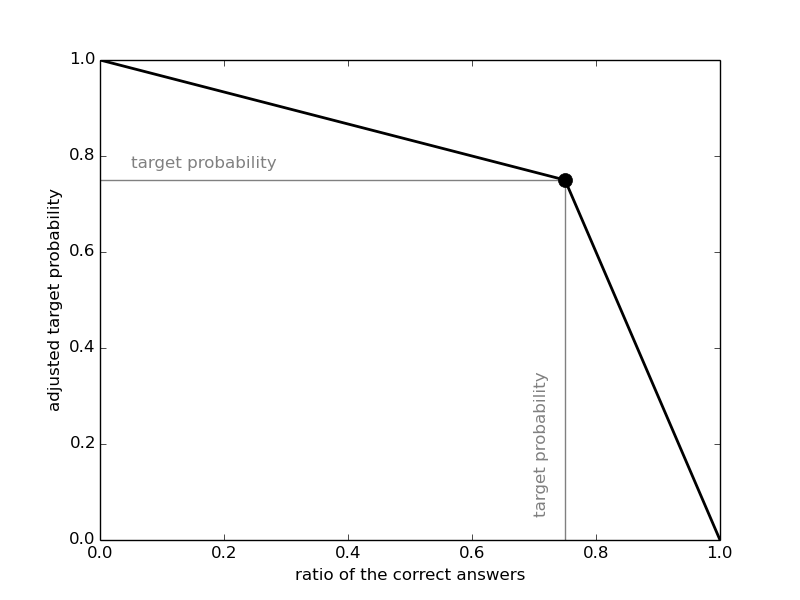
\includegraphics[width=\textwidth]{target_probability_adjustment}
\end{frame}
% ------------------------------------------------------------------------------
% --------------------------- SLIDE --------------------------------------------
\begin{frame}
	\frametitle{Research Questions}
	\begin{itemize}
		\item<1-5> Does the adaptability have any effect?
			\begin{itemize}
				\item motivation vs. learning
			\end{itemize}
		\item<2-5> What are the optimal parameters (algorithm) for adaptivity?
			\begin{itemize}
				\item target difficulty, difficulty adjustment, items in options
			\end{itemize}
		\item<3-5> What is the effect of feedback loop?
			\begin{itemize}
				\item predictive model vs. question construction
			\end{itemize}
		\item<4-5> What is the impact of predictive model itself?
		\item<5> Can we reproduce lab based experiments in online environment?
	\end{itemize}
\end{frame}
% ------------------------------------------------------------------------------
% --------------------------- SLIDE --------------------------------------------
\begin{frame}
	\frametitle{User's Motivation: Target Item and Options}
	\begin{center}
		\begin{tabular}{llc}
			\toprule
			\head{Target item~~~~} & \head{Options~~~~} & \head{Answers}\\
			\midrule
			adaptive	& adaptive & $33.0$\\
			adaptive	& random & $20.0$\\
			random & adaptive	& $20.0$ \\
			random & random & $19.5$\\
			\bottomrule
		\end{tabular}
	\end{center}
\end{frame}
% ------------------------------------------------------------------------------
% --------------------------- SLIDE --------------------------------------------
\begin{frame}
	\frametitle{User's Motivation: Difficulty Adjustment}
	\begin{center}
		\begin{tabular}{llc}
			\toprule
			\head{Adjustment~~~~} & \head{Answers}\\
			\midrule
				true & $28.0$\\
				false & $21.0$\\
			\bottomrule
		\end{tabular}
	\end{center}
\end{frame}
% ------------------------------------------------------------------------------
% --------------------------- SLIDE --------------------------------------------
\begin{frame}
	\frametitle{Publications}
	\bibliographystyle{amsalpha}
	\nocite{*}
	\bibliography{bibliography}
\end{frame}
% ------------------------------------------------------------------------------
% --------------------------- SLIDE --------------------------------------------
\begin{frame}
	\frametitle{User's Motivation: Difficulty}
	\begin{center}
		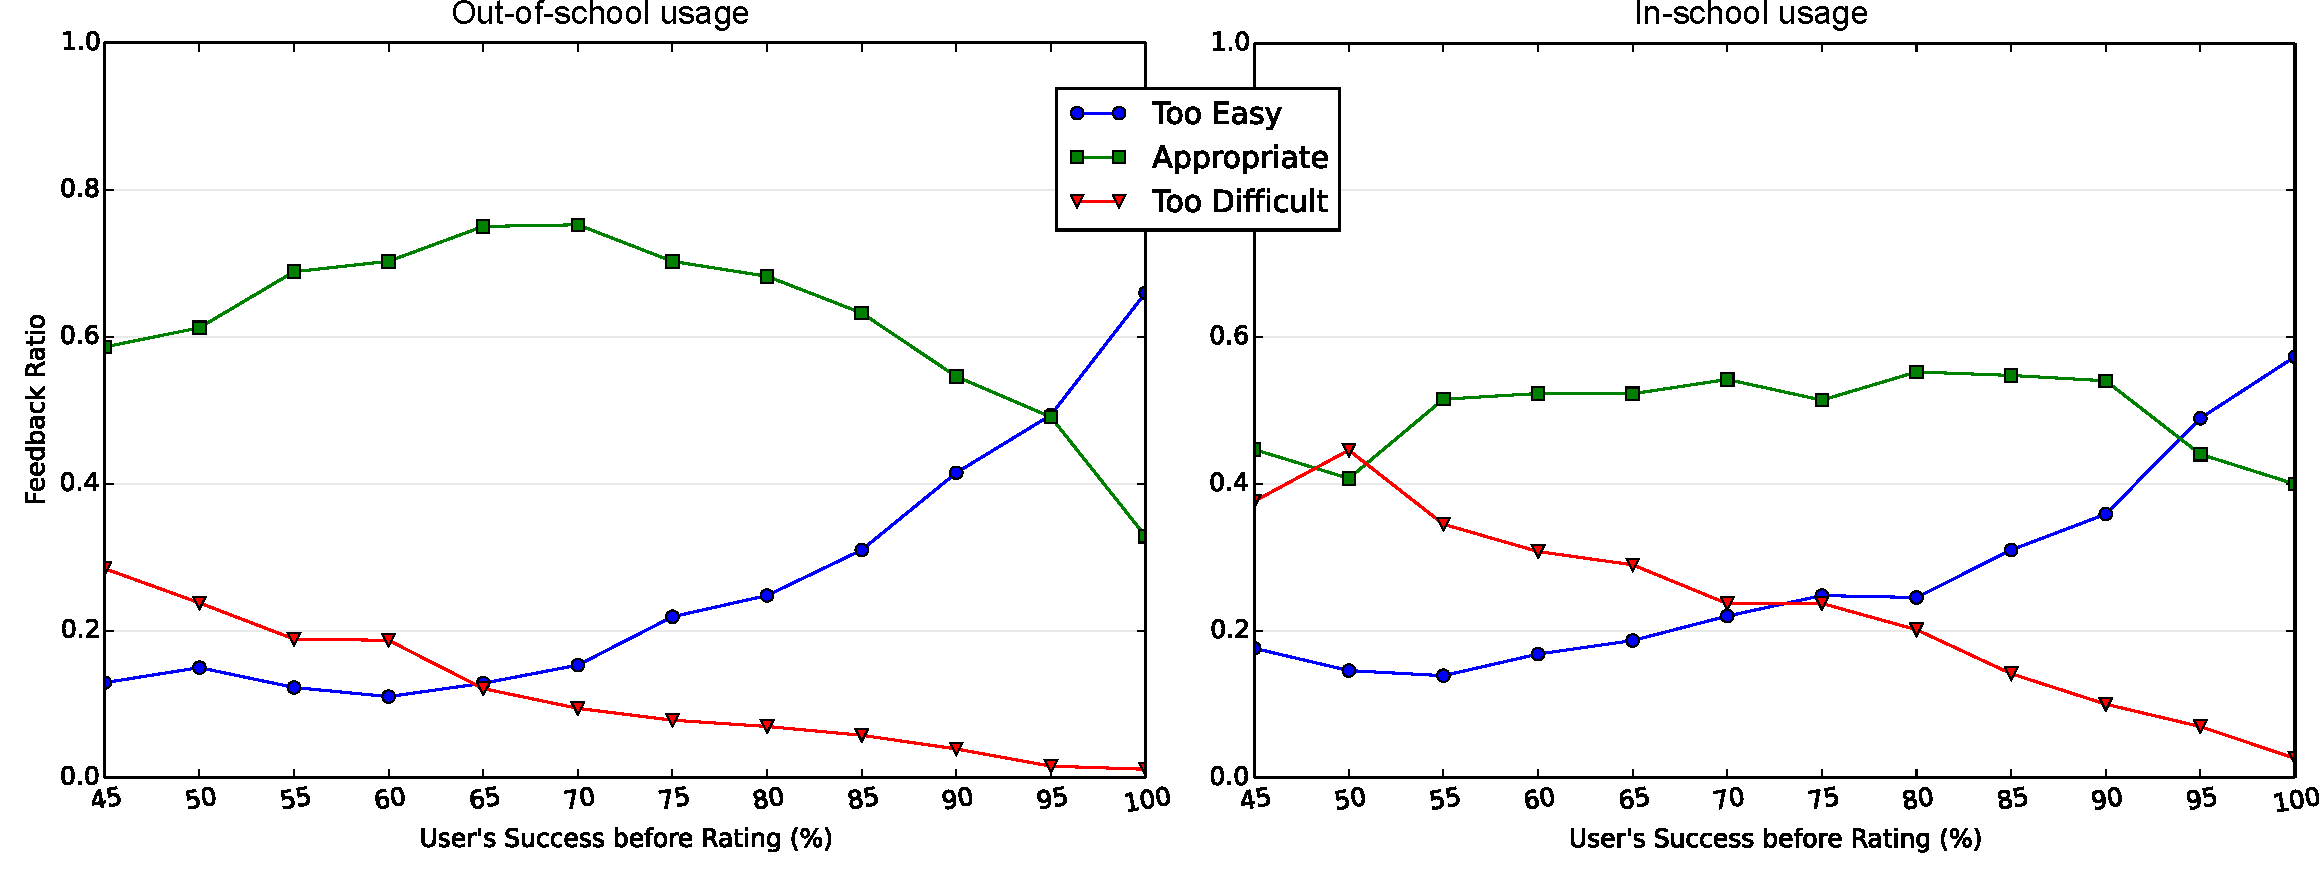
\includegraphics[width=\textwidth]{feedback}
	\end{center}
\end{frame}
% ------------------------------------------------------------------------------
% --------------------------- SLIDE --------------------------------------------
\begin{frame}
	\frametitle{Impact of Predictive Model on Student's Practice}
	\begin{center}
		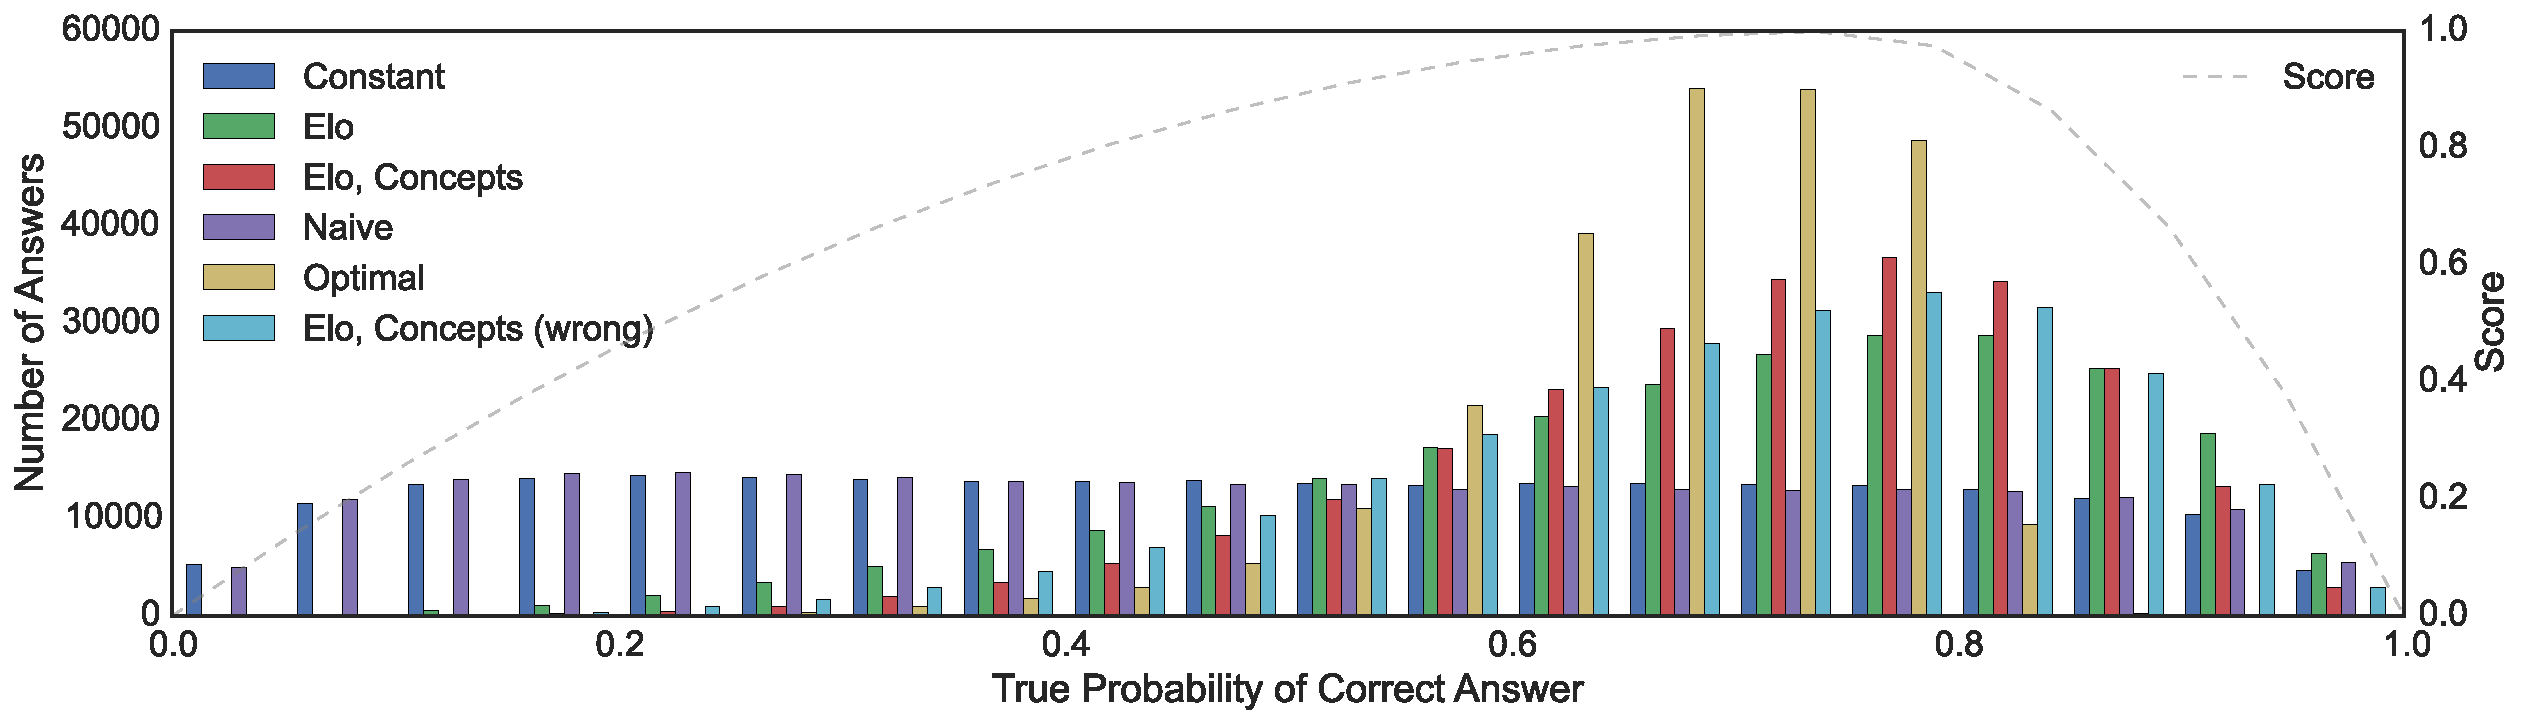
\includegraphics[width=\textwidth]{number_of_answers}
	\end{center}
\end{frame}
% ------------------------------------------------------------------------------
\end{document}
